%=========================================================
\chapter{Modelo dinámico}	
\label{cap:modDinamico}

	Este capítulo describe en modelo dinámico del sistema. en el se detallan todos los escenarios de ejecución del sistema. La figura~\ref{fig:casosDeUso} muestra el diagrama general del sistema y sus sib sistemas, y la figura~\ref{fig:casosDeUsoDetalle} muestra todos los casos de uso del sistema. En este documento solo detallamos los casos de uso del subsistema de gestión de cursos.
	
\begin{figure}[htbp]
	\begin{center}
		\fbox{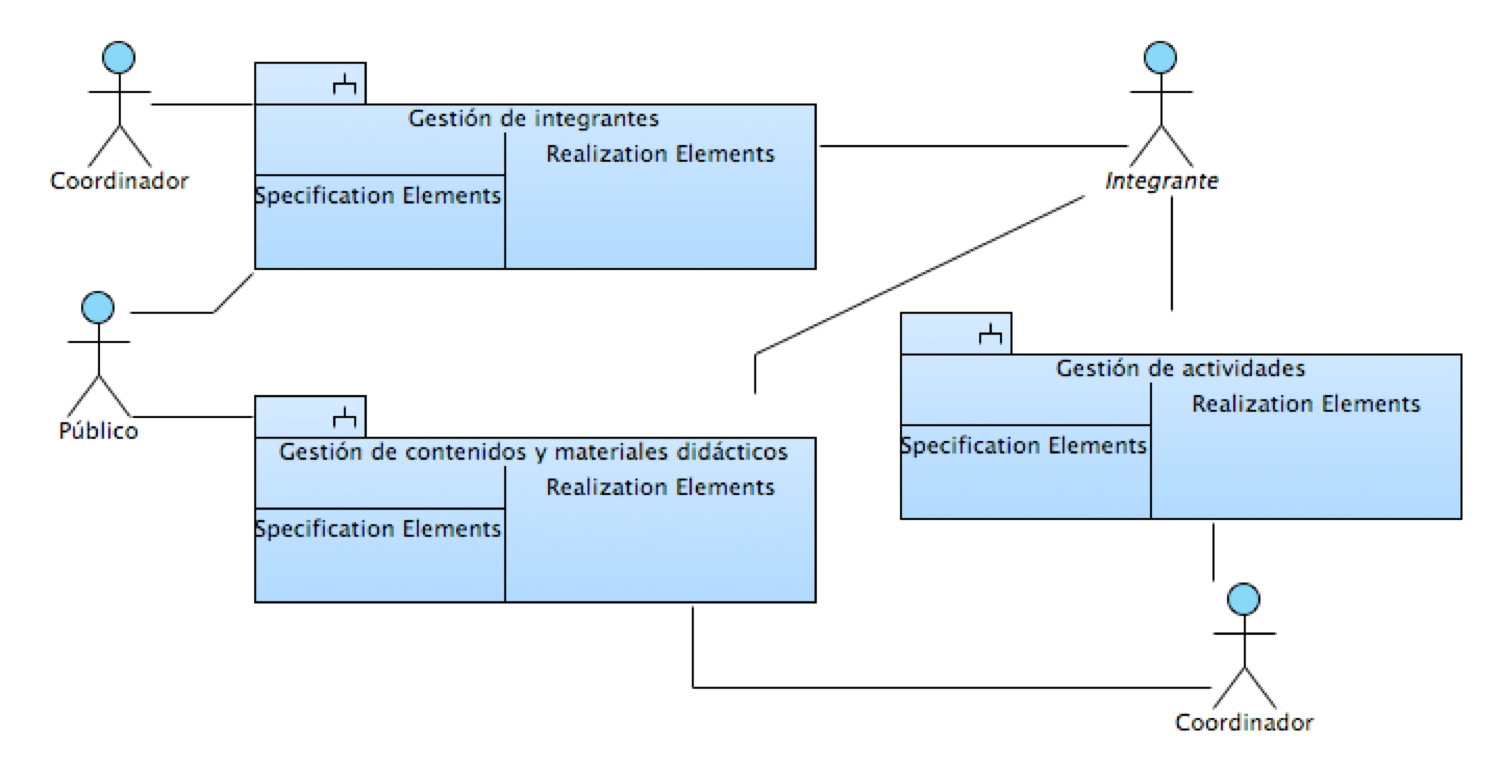
\includegraphics[width=.8\textwidth]{images/casosDeUso}}
		\caption{Diagrama de casos de uso del sistema.}
		\label{fig:casosDeUso}
	\end{center}
\end{figure}

\begin{figure}[htbp]
	\begin{center}
		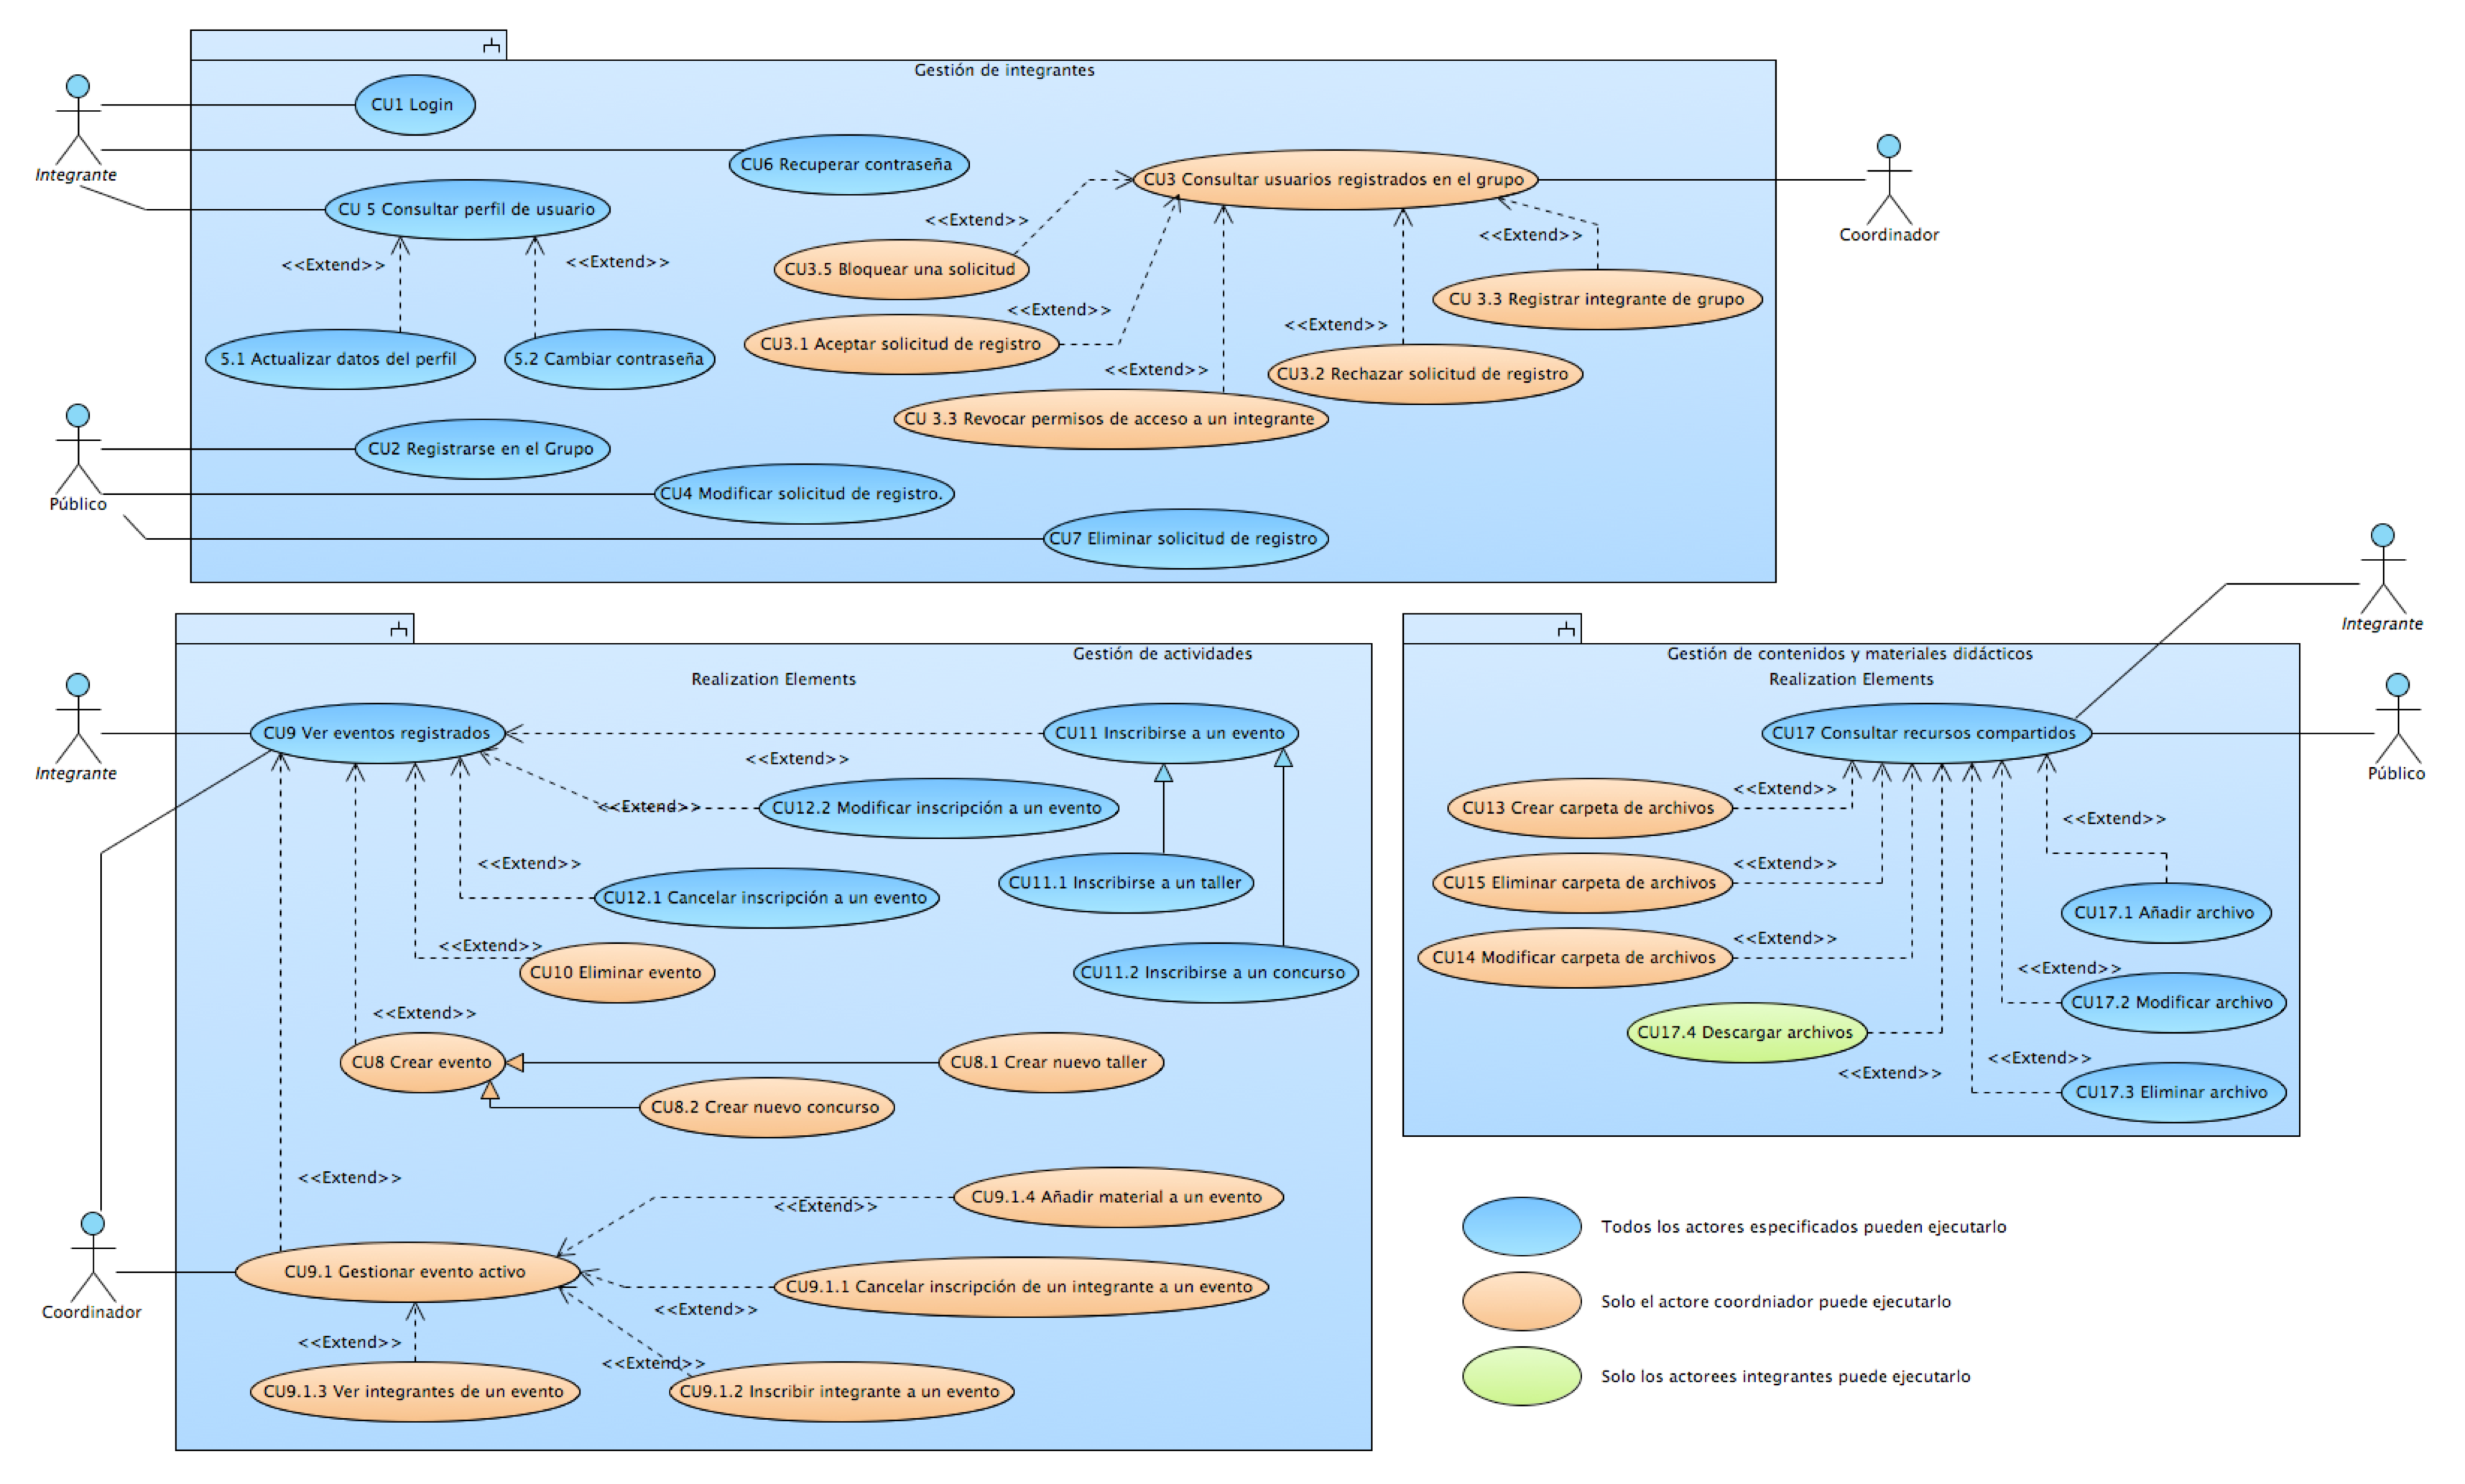
\includegraphics[angle=90, width=.7\textwidth]{images/casosDeUsoDetalle}
		\caption{Diagrama detallado del sistema.}
		\label{fig:casosDeUsoDetalle}
	\end{center}
\end{figure}

%---------------------------------------------------------
\section{Descripción de actores}

%---------------------------------------------------------
\begin{Usuario}{\hypertarget{getenteOperaciones}{\subsection{Gerente de Operaciones}}}{
	Es el encargado de todas las operaciones de la empresa y está por encima de los ejecutivos de producción y de ventas principalmente.
}
    \item[Responsabilidades:] \cdtEmpty
    \begin{itemize}
		\item Supervisar la operación.
		\item Plantear y supervisar el logro de las metas de la empresa y su crecimiento económico.
		\item ...
    \end{itemize}

	\item[Perfil:] \cdtEmpty
    \begin{itemize}
		\item Amplia experiencia en el ramo.
		\item Licenciatura como mínimo.
		\item ...
    \end{itemize}
\end{Usuario}

A continuación se detallan los casos de uso.

%---------------------------------------------------------
% CASOS DE USO

%======================================================================================
\begin{UseCase}{CU17}{Información del proyecto}{
		Permite al Lider de proyecto visualizar la información general del proyecto.
	}
		\UCitem{Actor}{\hyperlink{LiderProyecto}{Lider de proyecto}}
		\UCitem{Propósito}{Permitír al Lider de proyecto ver la información general del proyecto}
		\UCitem{Entradas}{\begin{itemize}
		\item Ninguna 
		\end{itemize}
.}
		\UCitem{Salidas}{Ninguna}
		\UCitem{Destino}{Pantalla de gestión de proyectos}
		\UCitem{Precondiciones}{Ninguna}
		\UCitem{Postcondiciones}{Ninguna}
		\UCitem{Errores}{Ningunó}
		\UCitem{Observaciones}{}
	\end{UseCase}
%--------------------------------------
	\begin{UCtrayectoria}{Principal}
		\UCpaso[\UCactor] Da click en el icono 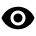
\includegraphics[height=10pt]{./images/iconos/ic_visibility_black_18dp.png}
        \UCpaso [\UCsist] accede a la pantalla \hyperref[fig:IU17]{IU17 Información del proyecto}. \label{item:CU17Item1} \Trayref{A}.
	\end{UCtrayectoria}

%--------------------------------------		
		\begin{UCtrayectoriaA}{A}{ El actor da click en el boton 'regresar'}
			\UCpaso [\UCsist] accde a la pantalla \hyperref[fig:IU09]{IU09 Gestionar Proyectos}.
		\end{UCtrayectoriaA}		
		
		
%-------------------------------------- TERMINA descripción del caso de uso.



